\documentclass[conference]{IEEEtran}
\usepackage{cite}
\usepackage{amsmath,amssymb,amsfonts}
\usepackage{graphicx}
\usepackage{textcomp}
\usepackage{xcolor}
\usepackage{booktabs}
\usepackage{listings}
\usepackage{hyperref}
\usepackage{cleveref}
% TikZ removed — all diagrams are now Typst-compiled PDFs

\begin{document}

\title{Grand Assembly of Computational Hard Problems: The Art of Agentic Coding}

\author{...}  % placeholder

\maketitle

\begin{abstract}
A unified library of polynomial-time reductions between NP-hard problems would let practitioners route any supported problem to a specialized solver---quantum hardware, commercial optimizers, or domain heuristics---through a single interface.
No such library exists, because building one by hand demands a shared formalism across many contributors and ongoing maintenance as the literature grows.
We address this gap with AI coding agents steered by \emph{skills}: versioned, composable workflow documents that encode project conventions and domain knowledge.
The approach yields a library of over 100 problem types, due to three changes.
(1)~A \emph{no-code contribution route} lets domain experts add reductions by filing structured issues; no familiarity with the implementation language is needed.
(2)~A \emph{multilayer verification stack} checks each reduction from type signatures through property-based tests to \emph{agentic feature tests}---automated agents that act as virtual users, exercising the library end-to-end.
(3)~A \emph{fully automated pipeline} lets one maintainer run the project, and a new maintainer can on-board in half a day.
The entire stack was built in ten weeks. The methodology shows that agents, given the right scaffolding, can produce verified software artifacts whose scope would be impractical to maintain by hand.
\end{abstract}

%======================================================================
%  SECTION 1: INTRODUCTION
%======================================================================
\section{Introduction}\label{sec:intro}

\subsection{The Problem: Many Hard Problems, Few Solvers}

Combinatorial optimization problems arise throughout science and engineering.
An airline needs to assign crews to flights.
A chip designer needs to allocate registers.
A logistics company needs to route delivery trucks.
Each of these is an instance of an NP-hard problem---a class of problems for which no efficient general-purpose algorithm is known, but which can be solved in practice for moderate sizes by specialized solvers.

The difficulty is that each solver speaks its own narrow language.
Rydberg atom arrays~\cite{lucas2014, pichler2018}---a type of quantum hardware---natively solve the Maximum Independent Set problem on geometric graphs.
D-Wave quantum annealers~\cite{glover2019} solve Quadratic Unconstrained Binary Optimization.
Commercial engines like Gurobi and CPLEX solve Integer Linear Programs.
A practitioner with a graph coloring problem cannot directly use any of these solvers without first \emph{translating} the problem into a form the solver understands.

This translation is called a \emph{reduction}: a polynomial-time algorithm that converts an instance of one problem into an instance of another, together with an inverse map that translates the solution back.
Reductions are the central tool of computational complexity theory~\cite{karp1972}, but they also have immediate practical value: each verified reduction is a bridge connecting a new problem to an existing solver.

\subsection{Bridging Problems to Solvers}

A single reduction bridges one problem to one solver.
To bridge \emph{many} problems to \emph{many} solvers, we organize reductions as a \emph{directed graph}.
Each node is a problem type (e.g., Satisfiability, Max-Cut, Traveling Salesman).
Each directed edge is a verified reduction---code that transforms instances forward and maps solutions back.
A path through the graph bridges any supported problem to any reachable solver.

\begin{figure*}[t]
  \centering
  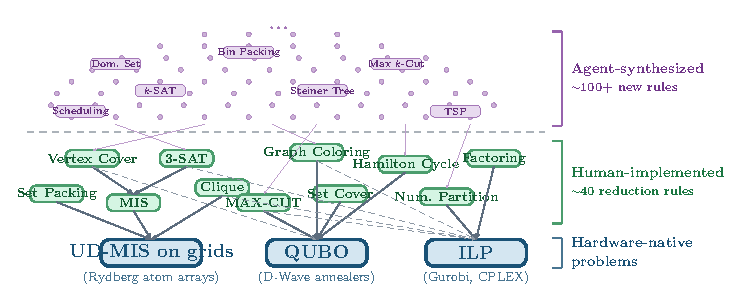
\includegraphics[width=0.88\textwidth]{figures/problemtree.pdf}
  \caption{The reduction graph connects 27~NP-hard problem types to three solver families through 45~verified transformation rules.
    \textbf{Bottom layer}: solvers---Maximum Independent Set on unit-disk graphs (UD-MIS) for Rydberg atom arrays, QUBO for D-Wave quantum annealers, and ILP for commercial solvers.
    \textbf{Middle layer}: 27~problem types with color-coded edges showing solver reachability.
    MIS is the dominant hub with 14~incoming and 13~outgoing edges.
    Each new edge creates composite paths through the entire graph.}
  \label{fig:reduction-graph}
\end{figure*}

The graph currently contains 27~problem types connected by 56~directed edges (\Cref{fig:reduction-graph}).
Reductions implemented independently compose automatically through the graph.
For example, one contributor implemented Factoring $\to$ Circuit Satisfiability, and another implemented Circuit Satisfiability $\to$ Integer Linear Programming.
Neither intended the composition, yet the graph enables factoring integers via linear programming by chaining the two reductions.
Each new edge creates not just one connection but new paths through the entire graph.

\subsection{The Challenge}

Building such a graph is itself a hard problem---not computationally, but organizationally.
Earlier attempts illustrate the difficulty.
QUBO-specific tools---PyQUBO~\cite{Zaman2021PyQUBO}, qubovert~\cite{Iosue2022qubovert}, ToQUBO.jl~\cite{Monteiro2022ToQUBO}, and D-Wave's Ocean SDK~\cite{DWaveOcean2023}---convert problems into a single target formulation but provide no inter-problem reductions and no inverse maps for solution extraction.
Lucas~\cite{lucas2014} catalogued Ising formulations for Karp's 21~problems, but the result is a paper, not composable code.
The Karp DSL~\cite{Zhang2022Karp} and REDNP~\cite{Creus2014REDNP} provide languages for writing and testing reductions, but are pedagogical tools with no solver integration.
ProblemReductions.jl~\cite{Liu2024ProblemReductions}, the most direct predecessor, implements 18~problem types in Julia with a reduction graph structure---but has remained small (3~contributors, 13~stars) after two years.
The pattern is consistent: each project covers a handful of problems, then stalls.
More broadly, the gap between \emph{known} and \emph{implemented} reductions has widened for decades.
Hundreds of reductions exist in the literature---Garey and Johnson~\cite{garey1979} alone catalogue over 300~NP-hard problems with reduction sketches---yet the largest software implementation covers fewer than 20.
The bottleneck was never mathematical knowledge; it was building and maintaining the software.

The reason is organizational, not technical.
The graph's value grows with every edge, but so does the cost of maintaining it.
Every edge must conform to the same conventions---same interface, same file layout, same test pattern---because this uniformity is what makes edges composable.
Maintaining such uniformity across many contributions is precisely what human teams cannot do at scale.
Conventions drift as contributors accumulate their own patterns.
The domain experts who know the reductions rarely write systems code, bottlenecking progress on the few who know both.
When a new reduction appears in the literature, the mathematician who understands it has no way to contribute it without learning the implementation language and the project's conventions.
And the repetitive verification cycle that each edge demands---coding, testing, documenting---exhausts even dedicated maintainers.

We call this a \emph{bridge problem}: software whose subtasks are homogeneous and formally verifiable, but whose scale exceeds what human teams can sustain.
AI coding agents, constrained by a multilayer verification stack, break through these barriers.
A domain expert who discovers a new reduction can contribute it by filing a structured issue---no code required---and agents handle the implementation, testing, and documentation.
The agent produces volume; verification ensures correctness.

\subsection{Contributions}

Over nine weeks, a single maintainer and AI agents produced a Rust library with 27~problem types, 45~reduction rules, and $>$95\% test coverage.
Our contributions are:
\begin{itemize}
  \item \textbf{The bridge problem concept}: a characterization of software projects where homogeneous, verifiable subtasks create scale barriers that agents can overcome (\Cref{sec:bridge}).
  \item \textbf{A verified reduction graph} connecting 27~NP-hard problem types to specialized solvers, with emergent compositionality through automatic path composition (\Cref{sec:graph}).
  \item \textbf{A skill-based methodology} for mathematical software engineering, encoding workflow knowledge as reusable, versioned scripts that decompose multi-file tasks into agent-executable steps (\Cref{sec:method}).
  \item \textbf{Quantitative evidence}: a 15:1 agent-to-human message ratio, a 75\% rejection rate on 322~batch-submitted proposals demonstrating the quality gate's selectivity, and a 9-week development timeline (\Cref{sec:evaluation}).
\end{itemize}

The rest of this paper is organized as follows.
\Cref{sec:bridge} defines bridge problems and the three barriers.
\Cref{sec:graph} presents the reduction graph as a case study.
\Cref{sec:method} describes the methodology.
\Cref{sec:evaluation} provides evidence.
\Cref{sec:related} surveys related work.
\Cref{sec:conclusion} discusses limitations and future directions.

%======================================================================
%  SECTION 2: BRIDGE PROBLEMS
%======================================================================
\section{Bridge Problems}\label{sec:bridge}

A \emph{bridge problem} is a software project whose subtasks are homogeneous and formally verifiable, but whose scale exceeds what human teams can sustain.
We identify three structural barriers that distinguish bridge problems from ordinary large projects.

\subsection{Three Barriers to Human-Scale Development}

\paragraph{Convention drift.}
A reduction library demands strict uniformity: every rule file follows the same naming convention, implements the same trait, includes the same test pattern, and produces the same documentation artifacts.
Human teams cannot maintain this discipline across hundreds of contributions.
Conventions drift, shortcuts accumulate, and style guides go unread.
In our approach, the project specification (\texttt{CLAUDE.md}) and reusable skills encode every convention as a machine-readable document.
The agent reads it on every invocation and never deviates---convention compliance becomes a property of the tool, not a discipline of the team.

\paragraph{Effort exhaustion.}
Each new problem type requires definitions, examples, reductions, tests, overhead formulas, and documentation.
Verifying each component one by one---running the same round-trip test for the 45th time, checking the same overhead formula against the same symbolic expressions---requires sustained, detail-oriented effort that no individual or small team can maintain indefinitely.
A niche mathematical library also lacks the user base to surface issues through organic community usage.
Agents execute the same verification loop without fatigue, and agentic feature tests---where an agent role-plays as a downstream user---provide the testing frequency that the community size cannot.

\paragraph{Knowledge discontinuity.}
Human maintainers graduate, change jobs, or lose interest.
New contributors face a steep onboarding curve: understanding the architecture, the conventions, the testing patterns, and the implicit knowledge accumulated over years.
Skills encode this knowledge in executable, versionable form.
A new maintainer does not need to reconstruct the original developer's mental model from scattered comments and commit messages---they invoke the same skills that produced the codebase.
The \texttt{dev-setup} skill configures the development environment; the \texttt{add-rule} skill encodes the complete workflow for adding a reduction.
Open-source contribution, traditionally gated by the ability to absorb a project's implicit culture, becomes gated only by domain knowledge.

\subsection{Verification Constrains Agent Output}\label{sec:verification-bridge}

The natural concern is correctness: how can agent-written mathematical software be trusted?
Our answer is that contributor-specified ground truth flows through a verification stack that constrains what agents can produce.

\begin{figure}[t]
  \centering
  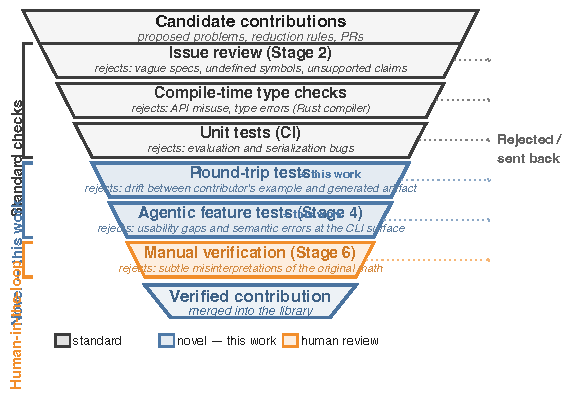
\includegraphics[width=\columnwidth]{figures/verification-funnel.pdf}
  \caption{Verification funnel.
    Agent-generated code is progressively filtered: the type system rejects structural errors, round-trip tests reject semantic errors, overhead validation rejects incorrect complexity claims, and agentic feature tests reject usability issues.
    Only code matching contributor-specified ground truth survives.}
  \label{fig:verification-funnel}
\end{figure}

A contributor supplies the creative elements that define correctness: formal problem definitions, worked examples with known solutions, and expected overhead formulas.
These flow through four verification layers:
\begin{enumerate}
  \item \textbf{Type system}: the Rust compiler rejects structural errors---wrong return types, missing inverse maps, references to nonexistent problem attributes---at compile time.
  \item \textbf{Round-trip tests}: for each reduction, a small instance is transformed forward, solved by brute force, mapped back, and verified optimal for the source. This catches the most mathematically subtle errors without per-reduction test logic.
  \item \textbf{Overhead validation}: symbolic size expressions are evaluated against actual target sizes, catching formula errors that are type-correct but mathematically wrong.
  \item \textbf{Agentic feature tests}: an agent reads the documentation, exercises the feature through the CLI, and judges whether results are consistent with domain knowledge---replacing the community feedback loop that niche libraries lack.
\end{enumerate}

The agent has freedom in \emph{how} to implement; verification eliminates freedom in \emph{what} the result must be.
Agent output $\subseteq$ contributor intent.

\subsection{Other Candidate Domains}

NP-hard reductions are not the only bridge problem.
Algorithm libraries, compiler optimization passes, numerical linear algebra routines, and hardware description languages share the same structure: homogeneous subtasks, formal correctness criteria, and a scale that exceeds what small teams can sustain.
In each case, domain experts can encode the ``how'' into reusable skills while the ``what'' remains a human judgment call.
The methodology does \emph{not} generalize to heterogeneous tasks---the staple of SWE-Bench---where each issue is structurally unique and resists skill-based decomposition.

%======================================================================
%  SECTION 3: CASE STUDY --- THE REDUCTION GRAPH
%======================================================================
\section{Case Study: The Reduction Graph}\label{sec:graph}

\subsection{What Is a Reduction?}

A \emph{reduction} from problem~$A$ to problem~$B$ is a pair of functions: a \emph{forward map} that transforms any instance of~$A$ into an instance of~$B$ in polynomial time, and an \emph{inverse map} that converts any solution of the $B$-instance back into a solution of the original $A$-instance.
If the reduction is correct, the extracted solution is optimal (or satisfying) for the original problem.

For example, the complement relationship between Minimum Vertex Cover (MVC) and Maximum Independent Set (MIS) gives a simple reduction: given a graph, the vertex cover problem asks for the smallest set of vertices that touches every edge, while the independent set problem asks for the largest set of vertices with no edges between them.
A set~$S$ is independent if and only if its complement $V \setminus S$ is a vertex cover, so the forward map is the identity (the same graph), and the inverse map complements the solution.
This 96-line implementation connects MVC to every solver reachable from MIS.

\subsection{Graph Structure}\label{sec:graph-structure}

We organize reductions into a directed graph $G = (V, E)$, where each vertex $v \in V$ represents an NP-hard problem type and each directed edge $(u, v) \in E$ represents a verified reduction from problem~$u$ to problem~$v$.
The graph contains 27~vertices (problem types) and 56~directed edges: 45~hand-coded reduction rules plus 11~edges inferred from subtype relationships (e.g., MIS on a geometric subgraph can always be treated as MIS on a general graph, because the geometric structure is a special case).

Three problems serve as ``compilation targets,'' each corresponding to a class of specialized solvers (\Cref{fig:reduction-graph}, bottom layer):
\begin{itemize}
  \item \textbf{MIS} (Maximum Independent Set): target for Rydberg atom arrays, which solve MIS natively on geometric graphs.
  \item \textbf{QUBO} (Quadratic Unconstrained Binary Optimization): target for D-Wave quantum annealers.
  \item \textbf{ILP} (Integer Linear Programming): target for commercial solvers like Gurobi and CPLEX.
\end{itemize}
MIS is the dominant hub with 14~incoming and 13~outgoing edges, reflecting its role as both a hardware target and an intermediary.
ILP, with 11~incoming edges, functions as a universal algebraic target.
A path from any problem to one of these targets provides a route to the corresponding solver.

\subsection{Emergent Compositionality}\label{sec:compositionality}

The graph's most valuable property is that independently implemented reductions compose automatically to solve problems that no single reduction was designed for.

Consider the problem of integer factoring---decomposing a number $N$ into its prime factors.
The Factoring $\to$ CircuitSAT reduction (272~lines of code) constructs a Boolean circuit representing an array multiplier: two bit-vector inputs $p$ and $q$, a grid of full-adder cells computing their product, and output constraints fixing the result to~$N$.
Any satisfying assignment to this circuit yields factors of~$N$.

Separately, the CircuitSAT $\to$ ILP reduction (225~lines) linearizes a Boolean circuit into integer constraints, encoding each logic gate as a set of linear inequalities.

Neither reduction was designed with the other in mind---they were implemented in separate pull requests, weeks apart.
Yet the graph infrastructure enables automatic chaining: given a Factoring instance, the system finds the path Factoring $\to$ CircuitSAT $\to$ ILP, applies both reductions in sequence, solves the resulting integer program with a commercial solver, and extracts the factors by composing the inverse maps in reverse order.
This works because every reduction provides type-safe solution extraction through a common interface, and the path-finding algorithm composes extractors automatically.

Each new edge amplifies the graph.
Adding a single reduction from problem~$X$ to MIS does not just connect $X$ to MIS---it connects $X$ to every solver reachable from MIS, and it connects every problem with a path to~$X$ to MIS.
This multiplier effect---where value grows faster than the number of edges---justifies the investment in verified reduction infrastructure over ad-hoc, one-off transformations.

\subsection{Verification by Round-Trip Testing}\label{sec:roundtrip}

How do we know each reduction is correct?
Every reduction admits a fully automatable correctness test that requires no problem-specific oracle.
The test, which we call \emph{round-trip testing}, works as follows:

\begin{enumerate}
  \item Construct a small source instance (e.g., a graph with 5--8 vertices).
  \item Apply the forward map to produce a target instance.
  \item Solve the target by brute-force enumeration (feasible for small instances).
  \item Apply the inverse map to extract a solution for the source.
  \item Verify that the extracted solution is optimal for the source (also by brute force).
\end{enumerate}

This pattern is the same for all 45~reductions.
It catches the most mathematically subtle errors---incorrect variable mappings, off-by-one indexing in literal-to-vertex transformations, forgotten negations---without requiring a human to write problem-specific test logic.

The library's type system enforces this pattern structurally: the \lstinline{ReduceTo<T>} trait requires both a forward map and an inverse map in a single implementation.
An agent cannot compile a forward reduction without providing solution extraction.
See \Cref{app:architecture} for the complete type architecture.

%======================================================================
%  SECTION 4: METHODOLOGY
%======================================================================
\section{Methodology}\label{sec:method}

The central design challenge is separating \emph{creative} decisions from \emph{routine} execution.
Adding a reduction to the graph requires answering questions that only a domain expert can answer: which problem is industrially relevant and worth adding?
What is the formal definition?
Which small example would be both illustrative and sufficient to check correctness?
What is the polynomial overhead?
Everything else---writing Rust code, constructing tests, generating documentation, fixing CI---is routine work that follows a fixed pattern regardless of the mathematical content.

Our answer is a pipeline of \emph{progressive quality gates} built around this separation.
The creative elements are captured in structured issue templates---one for models, one for rules---whose fields correspond exactly to the questions above.
The \texttt{propose} skill helps contributors fill in these fields interactively, asking one question at a time in mathematical language.
Once the creative decisions are recorded, the remaining stages are fully automated.

\subsection{From Contributor to Verified Code}\label{sec:pipeline-overview}

The pipeline has five stages, each backed by one or more \emph{skills}---persistent, versioned markdown documents that decompose complex tasks into numbered agent-executable steps (\Cref{fig:pipeline}).

\begin{figure}[t]
  \centering
  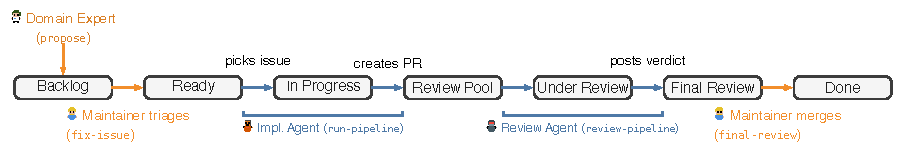
\includegraphics[width=\columnwidth]{figures/pipeline.pdf}
  \caption{Contribution pipeline from proposal to merged code.
    Orange transitions require human judgment (selecting work and approving results); blue transitions are fully automated by skills.
    Each stage independently validates before passing to the next.}
  \label{fig:pipeline}
\end{figure}

\textbf{Stage~1: Propose.}
A domain expert---who need not know the codebase or even the programming language---provides the creative elements that only a human can supply.
Two paths are available.
The \texttt{propose} skill guides the contributor interactively, asking one question at a time in mathematical language: what is the motivation, what is the formal definition, what is a small example that exercises the core structure?
Alternatively, the contributor fills in a structured GitHub issue template directly---the template fields mirror the same creative questions.
Either way, the output is an issue whose fields capture every creative decision needed for implementation.

Crucially, the agent first analyzes the graph's topology to identify the most valuable contributions (\Cref{app:topology}).
Three categories guide the analysis:
\emph{orphan nodes}---problem types with no reductions to or from any other node;
\emph{redundant rules}---direct reductions dominated by a cheaper composite path;
and \emph{missing proof paths}---problems with no reduction chain from 3-SAT.
The agent ranks proposals by priority: rules that connect orphans or fill proof-chain gaps are suggested first.
Before filing the issue, the agent runs the quality checks from Stage~2 on the draft, catching problems before they reach review.

\textbf{Stage~2: Validate.}
The \texttt{check-issue} skill applies four independent tests to every proposal: \emph{usefulness} (does a reduction path already exist? is this one dominated by a cheaper composite path?), \emph{non-triviality} (is this a genuine structural transformation, not a variable substitution?), \emph{correctness} (do the cited references exist and support the claims?), and \emph{writing quality} (are all symbols defined, all template sections complete, all examples fully worked?).
References are verified through a fallback chain: project bibliography, then web search---never hallucinated.
Only proposals passing all four checks receive a \texttt{Good} label and proceed.

\textbf{Stage~3: Implement.}
The \texttt{issue-to-pr} skill converts a validated issue into a pull request.
It enforces a strict \emph{one item per PR} rule: a reduction rule cannot be bundled with its source model, because the model must exist on main before the rule can be tested.
The skill reads the issue and all its comments, researches references to resolve ambiguities, generates an implementation plan, and dispatches to the appropriate implementation skill (\texttt{add-model} or \texttt{add-rule}).
Each implementation skill encodes a complete checklist---9~items for rules, 11~for models---that must be satisfied before any code is written.

\textbf{Stage~4: Review.}
Two parallel sub-agents, each operating in a fresh context window, review the implementation: one checks structural completeness (file registration, macro usage, test coverage), the other checks code quality and semantic correctness against the original issue specification.
Fresh context prevents the confirmation bias that arises when an agent reviews its own work.
CI failures trigger up to three automated fix-and-retry cycles.

A third review layer---\emph{agentic feature testing}---simulates a downstream user.
An agent reads the documentation, installs the library, exercises the new feature through the CLI, and judges whether the results are consistent with its domain knowledge.
This replaces the community feedback loop that open-source projects normally rely on: rather than waiting for users to discover issues post-release, agent-users test the feature before merge.
The CLI design is essential here---because agents and humans share the same command-line interface, the agent tests exactly what a real user would invoke.
Unlike unit tests (which verify internal correctness), agentic feature tests verify that the feature is \emph{usable}: that the documentation is accurate, that the CLI output is interpretable, and that the reduction produces results consistent with the agent's knowledge of the underlying mathematics.

\textbf{Stage~5: Merge.}
The maintainer makes the final quality judgment and merges.
This is one of only two human decisions in the pipeline; the other is moving an issue from Backlog to Ready (Stage~3).

\paragraph{Three agent roles.}
The pipeline uses agents in three distinct roles, each backed by a set of skills.

\emph{Mentors} (4~skills) interact with humans.
%
\begin{center}
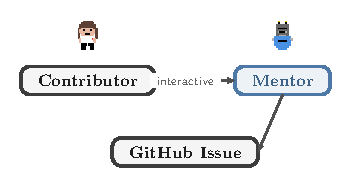
\includegraphics[height=1.8cm]{figures/role-mentor.pdf}
\end{center}
%
\noindent
The \texttt{propose} skill conducts an interactive session in mathematical language, asking one question at a time: what is the problem, what is the formal definition, what does a worked example look like?
Before filing, it pre-validates the draft against Stage~2's quality checks.
The \texttt{fix-issue} skill brainstorms with contributors to resolve quality problems.
The \texttt{final-review} skill guides the maintainer through merge decisions.
The \texttt{dev-setup} skill onboards new developers.

\emph{Orchestrators} (12~skills) know less than the human about \emph{what} should be built, but execute routine heavy-lifting that follows fixed patterns.
%
\begin{center}
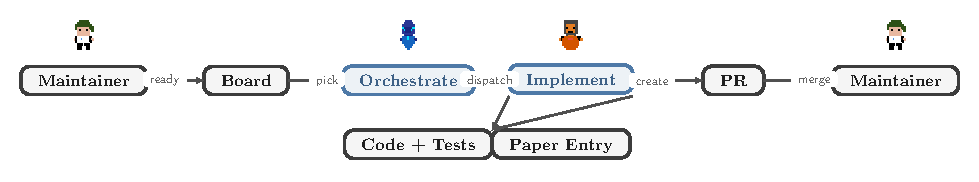
\includegraphics[width=\columnwidth]{figures/role-worker.pdf}
\end{center}
%
\noindent
Orchestration workers manage the pipeline headlessly: \texttt{project-pipeline} picks the highest-ranked Ready issue, creates an isolated git worktree, dispatches an implementation worker, and moves the result to the review queue; \texttt{review-pipeline} addresses code-review comments, runs agentic feature tests, and retries CI failures.
Implementation workers produce artifacts: \texttt{add-model} and \texttt{add-rule} write code following skill checklists; \texttt{write-model-in-paper} and \texttt{write-rule-in-paper} generate paper entries with proof sketches and worked examples.
Quality workers validate against rubrics: \texttt{check-issue} validates proposals before implementation; \texttt{review-implementation} dispatches parallel sub-agents in fresh context to review code; \texttt{fix-pr} resolves CI failures and review comments.
\texttt{release} handles version bumps and publishing.
The maintainer makes exactly two decisions in the entire pipeline: moving an issue from Backlog to Ready, and merging the final pull request.

\subsection{Why Skills, Not Prompts or Scripts}\label{sec:skills}

Traditional automation---Makefiles, CI pipelines, shell scripts---is \emph{mechanical}: every step is predetermined, and human involvement is impossible mid-execution.
Skills are a different kind of automation: \emph{abstract}.
A skill defines \emph{what} must happen (validate references, construct an example, write a proof sketch) without fixing \emph{how}.
When the task is routine, the agent executes autonomously.
When the task requires creativity or deep judgment---choosing which example best reveals correctness, deciding whether a proposed reduction is non-trivial---the skill can pause and involve a human as a resource, then resume.
The same skill thus operates headlessly in the pipeline (\texttt{make run-pipeline}) and interactively with a contributor (\texttt{propose}), adapting its execution mode to the context.

Skills also differ from per-invocation prompts in three ways that matter for sustainability.

\emph{Skills are versioned.}
They are committed to the repository and evolve through pull requests, just like code.
A bug in a skill is fixed once and benefits all future invocations.
A per-invocation prompt must be re-crafted each time, and improvements are lost.

\emph{Skills are compositional.}
Orchestration skills invoke implementation skills, which invoke quality gates.
A single \texttt{project-pipeline} command triggers the full cascade---pick a task from the project board, create an isolated workspace, validate the issue, implement, test, review, document, and produce a pull request.
The maintainer's effort scales with the number of \emph{skill types}, not the number of tasks.

\emph{Skills encode domain knowledge that cannot be inferred from code.}
The \texttt{add-rule} skill specifies that overhead expressions must use getter methods matching the source type, that examples must have a \lstinline{pub fn run()} entry point, and that the paper entry requires a proof sketch.
An agent reading only the codebase might infer some conventions but would miss others---the skill makes all conventions explicit.

The library comprises 14~skills in six categories: orchestration~(3), community contribution~(1), implementation~(2), quality gates~(4), documentation~(2), and onboarding~(2).

\begin{figure}[t]
\centering
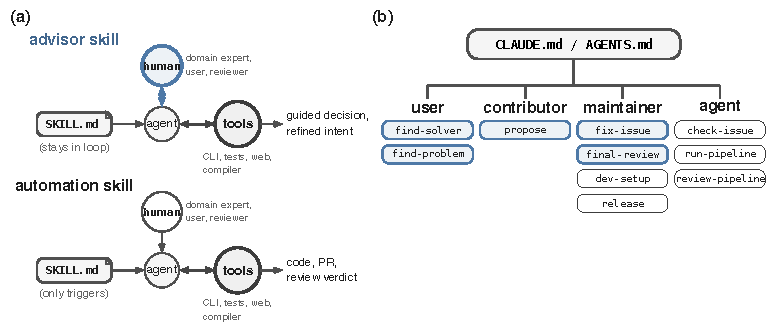
\includegraphics[width=\columnwidth]{figures/skill-map.pdf}
\caption{Project knowledge architecture.
  \texttt{CLAUDE.md} defines conventions, architecture, and commands;
  skills in four categories encode reusable workflows that reference it.
  Inner nodes show key source directories the skills operate on.}
\label{fig:skill-architecture}
\end{figure}

\subsection{Correctness by Construction}\label{sec:verification}

Correctness assurance comes from a seven-layer verification stack (\Cref{app:verification}).
The key insight is that different layers catch different classes of errors, and no single layer suffices.

\textbf{Layers~1--2} (type system and unit tests) catch structural errors cheaply.
The type system prevents entire categories of mistakes: an agent cannot implement a reduction without providing solution extraction, reference nonexistent problem attributes in overhead expressions, or omit required variant declarations.
These constraints are enforced at compile time by procedural macros that validate expression variable names against actual getter methods.

\textbf{Layer~3} (round-trip tests, described in \Cref{sec:roundtrip}) is the workhorse, catching the most mathematically subtle errors---incorrect variable mappings, off-by-one indexing, forgotten negations---without per-reduction test logic.

\textbf{Layer~4} (overhead validation) compares symbolic size expressions against actual target sizes.
An agent might implement a correct reduction but declare the wrong overhead formula.
This layer catches formula errors that are type-correct but mathematically wrong.

\textbf{Layer~5} (materialized fixtures) addresses the ``lazy agent'' problem: agents that modify expected test outputs to make tests pass rather than fixing implementations.
Ground-truth data is generated independently and committed separately; tampering produces a visible diff in a file outside the agent's normal scope.

\textbf{Layers~6--7} (fresh-context review and documentation) catch errors invisible to automated tests.
Parallel sub-agents operating in fresh context windows prevent confirmation bias.
Proof sketches force articulation of mathematical arguments; a completeness checker ensures every graph edge is documented.

The skill system ensures all seven layers are invoked for every task.
Without skills, an agent might skip overhead validation or omit the paper entry---errors that would accumulate silently over many contributions.

\subsection{Why Rust?}\label{sec:why-rust}

The choice of implementation language has outsized impact in agentic workflows, because the agent's edit--compile--test loop runs hundreds of times per session.
None of the maintainers had written Rust before this project---the language was chosen for properties that benefit agents, not developers.

\emph{Explicit, actionable error messages.}
The Rust compiler produces diagnostics that include the error location, the conflicting types or lifetimes, and often a suggested fix.
Agents parse these messages and resolve errors without human intervention---a property we rely on throughout the pipeline.
Languages with less structured diagnostics (e.g., C++ template errors) would require more agent reasoning per cycle.

\emph{Fast feedback.}
Incremental compilation and the built-in test harness produce results in seconds.
A typical round-trip test compiles and runs in under 3~seconds, enabling agents to iterate rapidly.
High feedback rate---short cycles between edit and result---is the single most important factor in agent productivity.

Rust's well-known strengths---memory safety eliminating entire bug categories at compile time, high performance, a 7\,MB binary, and Cargo's integrated toolchain---further reduce the surface area of errors agents must debug.
Procedural macros deserve special mention: they enable the compile-time validation of overhead expressions and variant registrations that powers Layers~1 and~4 of the verification stack.

%======================================================================
%  SECTION 5: EVIDENCE
%======================================================================
\section{Evidence}\label{sec:evaluation}

We evaluate through development metrics from the project's history, an analysis of the automated quality gate, and case studies showing how verification layers interact.
All development used Claude Code~\cite{Anthropic2025ClaudeCode} with Claude models (Sonnet~3.5 and Sonnet~4; the model version evolved during development).
Skills are plain markdown documents portable to any coding agent.

\subsection{Development Metrics}\label{sec:metrics}

The repository contains 59~merged pull requests and 253~commits on main spanning nine weeks (January~9 to March~13, 2026), authored by four contributors.
Session metadata across 283~agent sessions (300~MB of conversation transcripts) reveals the scale of agent involvement: 9,429~assistant messages in response to 630~user messages---a \textbf{15:1 automation amplification ratio}.
The average session involved 5.8~user messages and 51~tool calls, with measured wall-clock time totaling 115~hours across 108~sessions with timing data.

\begin{table}[t]
\caption{Codebase growth timeline.}\label{tab:growth}
\centering
\small
\begin{tabular}{@{}lcccc@{}}
\toprule
Date & Models & Rules & Tests & Examples \\
\midrule
Jan 10 (initial) & 17 & 0 & 0 & 0 \\
Jan 26 (feature parity) & 20 & 22 & 0 & 1 \\
Feb 15 (arch.\ redesign) & 21 & 44 & 101 & 35 \\
Mar 13 (current) & 27 & 45 & 114 & 45 \\
\bottomrule
\end{tabular}
\end{table}

\begin{figure}[t]
  \centering
  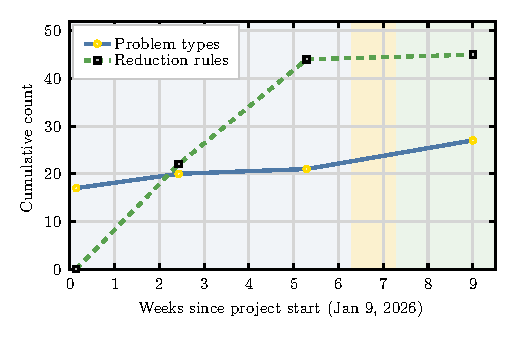
\includegraphics[width=\columnwidth]{figures/timeline.pdf}
  \caption{Cumulative growth of problem types and reduction rules over nine weeks.
    Background bands mark three development phases: manual (Phase~1), basic skills (Phase~2), and full pipeline (Phase~3).
    Background bands mark three development phases.}
  \label{fig:timeline}
\end{figure}

\Cref{tab:growth} and \Cref{fig:timeline} trace the growth across three phases.
\textbf{Phase~1 (Manual, 35~PRs)}: no skills; the maintainer issued step-by-step commands and established the architecture.
\textbf{Phase~2 (Basic skills, 9~PRs)}: initial \texttt{add-model}/\texttt{add-rule} skills reduced per-task human involvement.
\textbf{Phase~3 (Full pipeline, 15~PRs)}: complete skill library with orchestration, quality gates, and multi-agent review.
The current codebase comprises 54,599~lines of Rust source, 28,343~lines of tests, and 6,362~lines of examples.

\paragraph{Interaction evolution.}
Analysis of 2,196~user prompts reveals a shift from imperative to declarative interaction as skills matured.
In Phase~1, prompts averaged 8--12 words (e.g., ``implement Satisfiability to MIS reduction'').
By Phase~3, 30\% of prompts were 1--3 words (e.g., ``\texttt{make run-pipeline}'').
This progression---from specifying actions to invoking skills---mirrors the classical shift from scripting to API design.

\paragraph{Observability.}
All pull requests are attributed to human GitHub accounts because the agent operates through the developer's local terminal.
Of 1,089~commits across all branches, 1,510~carry a \texttt{Co-Authored-By: Claude} trailer (the count exceeds total commits because branch commits are squash-merged on main).
This observability gap---the difficulty of distinguishing human-authored from agent-assisted work in git metadata---is itself a finding about current agentic workflows.

\subsection{Issue Quality Gate}\label{sec:quality-gate}

The \texttt{check-issue} skill was stress-tested when a contributor batch-submitted 414~issues---including 251~in a single day---proposing new reductions for the graph.
Of the 322~issues checked, only \textbf{81~(25\%) passed} all quality criteria (\Cref{tab:quality-gate}).

\begin{table}[t]
\caption{Issue quality gate results (322 checked).}\label{tab:quality-gate}
\centering
\small
\begin{tabular}{@{}lr@{}}
\toprule
Verdict & Count (\%) \\
\midrule
Good & 81 (25\%) \\
PoorWritten (incomplete specification) & 124 (39\%) \\
Wrong (factually incorrect) & 64 (20\%) \\
Trivial (obvious, adds no value) & 43 (13\%) \\
Useless (no practical application) & 18 (6\%) \\
\bottomrule
\end{tabular}
\end{table}

The \textbf{75\% rejection rate} demonstrates the necessity of automated quality gates in agentic pipelines.
Without \texttt{check-issue}, the pipeline would waste agent compute implementing incorrect or trivial reductions.
The most common failure was \emph{PoorWritten}---issues lacking complete mathematical specifications, making them unimplementable even by a skilled agent.
The \emph{Wrong} category~(20\%) included citations to non-existent papers, incorrect complexity claims, and reductions that do not actually preserve solution structure---errors that would be expensive to discover during implementation rather than at triage.

\subsection{Case Studies}\label{sec:cases}

\paragraph{Satisfiability $\to$ MIS (gadget construction).}
The classical Karp reduction~\cite{karp1972} works as follows.
Given a Boolean formula in conjunctive normal form (a conjunction of clauses, each a disjunction of literals), create one graph vertex per literal occurrence.
Add edges within each clause (so at most one literal per clause can be selected) and between complementary literals across clauses (so a variable cannot be both true and false).
A satisfying assignment corresponds to an independent set of size~$m$ (the number of clauses).
The implementation spans 171~lines.

This case illustrates how verification layers interact.
The number of edges in the constructed graph is worst-case \emph{quadratic} in the number of literals---but an agent might assume linear overhead.
Layer~4 (overhead validation) catches this by comparing symbolic expressions against actual target sizes.
Layer~3 (round-trip testing) catches a different class of error: off-by-one mistakes in literal-to-vertex mapping.
Both layers are necessary: correct indices with wrong overhead, or correct overhead with wrong indices, would each pass one layer but fail the other.

\paragraph{Factoring $\to$ CircuitSAT $\to$ ILP (emergent composition).}
As described in \Cref{sec:compositionality}, this chains two independently implemented reductions (272 + 225~lines) to factor integers via linear programming.
The Factoring $\to$ CircuitSAT step exercises the full verification stack: the multiplier circuit involves $\Theta(mn)$ full-adder cells (where $m$ and $n$ are the bit lengths of the two factors), and errors in carry propagation are caught by Layer~3 while overhead formula errors are caught by Layer~4.

\paragraph{MVC $\leftrightarrow$ MIS (trivial complement).}
At the opposite extreme, this 96-line reduction exploits the complement relationship described in \Cref{sec:graph} with identity overhead.
The pipeline's primary value here is enforcing conventions---file naming, macro registration, documentation---rather than catching logical errors.

%======================================================================
%  SECTION 6: RELATED WORK
%======================================================================
\section{Related Work}\label{sec:related}

\paragraph{AI coding agents.}
The evolution from SWE-agent~\cite{Yang2024SWEagent} and Devin~\cite{Wu2024Devin} to OpenHands~\cite{Wang2024OpenHands} and Claude Code~\cite{Anthropic2025ClaudeCode} has expanded single-task capabilities to 70--80\% on SWE-Bench~\cite{Xia2025LiveSWEagent}, but longer-horizon benchmarks reveal a capability cliff~\cite{Thai2025SWEEVO, Deng2025SWEBenchPro}.
Roychoudhury~\cite{Roychoudhury2025AgenticAI} identifies specification inference as the central difficulty.
Our approach structures work so each unit falls within the agent's reliable range, complementing architectural advances in agent design.

\paragraph{AI code maintainability concerns.}
A growing body of evidence suggests that unstructured AI-assisted coding creates maintenance burden rather than reducing it.
Analysis of an LLM-generated C~compiler found excessive abstraction layering, inclusion of rarely-useful features that increase bug surface area, and absent comments precisely where domain expertise matters most~\cite{Jones2026LLMCompiler}.
A study of 211~million changed lines found a 4$\times$ growth in code clones and a decline in refactored code from 24\% to 10\%, indicating that AI encourages copy-paste over sustainable architecture~\cite{GitClear2025CodeQuality}.
A difference-in-differences study of 807~AI-adopting repositories found persistent increases in code complexity despite transient velocity gains~\cite{CursorAI2025SpeedCost}, and a randomized controlled trial found experienced developers were 19\% \emph{slower} with AI tools on real tasks in their own repositories~\cite{Becker2025METRProductivity}.
Our skill-based framework is designed to address these concerns directly: skills enforce project conventions (naming, testing, documentation) at every invocation, versioned skill definitions prevent prompt drift, and seven-layer verification rejects non-conforming code before it enters the repository.
The agent never ``free-writes'' code---it follows a structured template that has been refined through pull requests, ensuring that generated code is as maintainable as hand-written code that follows the same conventions.

\paragraph{AI-discovered reductions.}
FunSearch~\cite{RomeraParedes2023FunSearch} and AlphaEvolve~\cite{Novikov2025AlphaEvolve} discover novel algorithms and reductions through evolutionary search, including improved bounds for combinatorial problems.
Jani\v{c}i\'{c}'s URSA~\cite{Janicic2025URSA} uses SAT-based constraint solving to verify reductions.
Our work is complementary: we implement and verify \emph{known} reductions; discovered reductions could feed into our pipeline as new issues.

\paragraph{Formal verification of generated code.}
VeriCoding~\cite{Bursuc2025VeriCoding} reports 27--44\% success on 12,504~formal specifications.
CLEVER~\cite{Thakur2025CLEVER} establishes hard Lean benchmarks.
VeriBench~\cite{Miranda2025VeriBench} finds self-optimizing agents approach 90\% compilation in Lean~4.
Mukherjee et al.~\cite{Mukherjee2025CoqPL, Mukherjee2025SynVer} demonstrate a two-LLM generate-then-verify pattern.
Our seven-layer stack trades full formal guarantees for practical effectiveness at the scale of 45~reductions.

\paragraph{Physics-inspired optimization.}
Schuetz et al.~\cite{Schuetz2022PhysicsGNN} solve QUBO at million-variable scale via graph neural networks.
He~\cite{He2024QuantumTSP} combines quantum annealing with GNNs for the Traveling Salesman Problem.
These approaches assume a QUBO or Ising formulation as input---precisely the transformation that our reduction graph provides as upstream infrastructure.

%======================================================================
%  SECTION 7: DISCUSSION AND CONCLUSION
%======================================================================
\section{Discussion and Conclusion}\label{sec:conclusion}

\subsection{Limitations}

\paragraph{Single case study.}
Evidence comes from one project by one primary developer.
Replication across independent projects and teams is needed.

\paragraph{Skill engineering cost.}
The 14~skills represent substantial upfront investment---iterative refinement across many agent sessions.
Each new domain requires its own skill engineering effort, though the methodology itself transfers.

\paragraph{Confounding factors.}
Both skills and underlying models improved during the nine-week span.
Temporal stratification across the three phases partially addresses this, but we cannot fully disentangle the two contributions.

\paragraph{Maintainer requirement.}
The pipeline is not fully autonomous: without human judgment at two transitions (selecting work and approving results), the system cannot determine what is worth building or whether results meet standards.
This is by design---but limits applicability to fully autonomous scenarios.

\subsection{Why Human Experts Remain Essential}

The pipeline's reliance on human judgment is not a temporary limitation awaiting better models---it reflects a fundamental gap.
LLMs do not perform genuine mathematical reasoning: performance drops up to 65\% when irrelevant clauses are added to otherwise identical problems~\cite{Mirzadeh2025GSMSymbolic}, reasoning models exhibit accuracy collapse beyond complexity thresholds~\cite{Shojaee2025IllusionOfThinking}, and multi-step compositional reasoning exhibits multiplicative error accumulation~\cite{Dziri2023FaithFate}.
Standard transformers are bounded by constant-depth threshold circuits (TC$^0$); even chain-of-thought extends expressiveness only to polynomial-time computation~\cite{Merrill2024ExpressivePower}.

The context window (200,000~tokens for Claude Opus~4.6) functions as working memory, not reasoning capacity: performance degrades 14--85\% as input length increases~\cite{Du2025ContextLengthHurts}, and LLMs cannot maintain internal state across turns~\cite{Huang2025LLMWorkingMemory}.
On research-level mathematics, the best models score below 2\% on FrontierMath~\cite{Glazer2024FrontierMath} and 8\% on Humanity's Last Exam~\cite{Paster2025HLE}.

Skills are our response: rather than encoding domain expertise in model weights (expensive retraining) or prompts (ephemeral), skills encode it in versionable documents that persist across sessions.
Creative decisions remain with humans; routine execution is delegated to agents.

\subsection{Future Work}

\paragraph{Industry impact.}
The reduction graph serves as a \emph{solver-agnostic compilation layer}.
Adding a single edge from a hardware platform's native formulation (e.g., MIS for Rydberg atoms) routes all 27~problem types to that device.
Each new problem added to the graph is instantly available on every connected solver.

\paragraph{Scaling to 100+ problems.}
The graph's value grows superlinearly: each new edge creates composite paths through the entire graph.
Three directions extend this work: composing with \emph{automated discovery} via evolutionary search~\cite{Novikov2025AlphaEvolve}, supplementing round-trip tests with \emph{formal verification} (machine-checked Lean or Coq proofs), and \emph{cost-aware path selection} where the optimal solver route depends on instance scale.

\subsection{Conclusion}

We have introduced \emph{bridge problems}---software projects whose scale exceeds human capacity but whose homogeneous, verifiable structure makes them amenable to agent execution constrained by systematic verification.
NP-hard problem reductions are the first convincing example: over nine weeks, a single maintainer and AI agents produced a verified reduction graph connecting 27~problem types to specialized solvers.

The core insight is that three structural barriers---convention drift, effort exhaustion, and knowledge discontinuity---make bridge problems infeasible for human teams, while verification ensures that agents cannot deviate from contributor-specified ground truth.
Skills encode workflow knowledge as reusable, versionable documents, lowering the contribution barrier from ``knows the programming language'' to ``knows the mathematics.''
As the graph scales toward 100+ problem types, it evolves from a library into a reduction compiler---a vision that is infeasible without agentic execution.

\bibliographystyle{IEEEtran}
\bibliography{references}

%======================================================================
%  APPENDICES
%======================================================================
\appendices

\section{System Architecture}\label{app:architecture}

The library's type system reduces the space of possible agent errors by making incorrect code fail to compile.
This appendix describes four mechanisms---the \texttt{Problem} trait, the \texttt{ReduceTo} trait, the \lstinline{#[reduction(overhead)]} macro, and the \lstinline{declare_variants!} registry---that enforce correctness structurally (\Cref{fig:architecture}).

\begin{figure}[t]
  \centering
  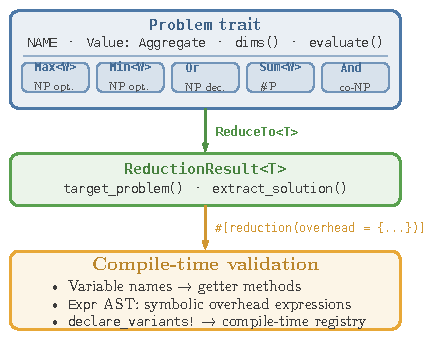
\includegraphics[width=\columnwidth]{figures/architecture.pdf}
  \caption{Trait hierarchy and compile-time validation.
    The \texttt{Problem} trait defines a universal evaluation interface; \texttt{ReduceTo<T>} requires both forward and inverse maps; procedural macros validate overhead expressions and variant registrations at compile time.}
  \label{fig:architecture}
\end{figure}

\paragraph{The Problem trait.}
Every problem type implements \texttt{Problem}, which requires: a constant name, an associated metric type (\texttt{SolutionSize<W>} for optimization problems, \texttt{bool} for decision problems), a method returning the configuration space dimensions, an \lstinline{evaluate()} method that scores any configuration, and variant metadata for type-parameter tracking.
The key member is \lstinline{evaluate()}: because every problem maps configurations to metrics through this uniform interface, a brute-force solver can enumerate the space and select the best solution, enabling the round-trip testing described in \Cref{sec:roundtrip} without problem-specific oracles.

\paragraph{The ReduceTo trait.}
The generic \lstinline{ReduceTo<T>} trait requires a \lstinline{reduce_to()} method returning a \texttt{ReductionResult} that bundles \lstinline{target_problem()} and \lstinline{extract_solution()}.
By requiring both forward and inverse in a single implementation, the type system ensures every reduction is round-trip capable---an agent cannot compile a forward reduction without providing the extraction logic.

\paragraph{Compile-time overhead validation.}
The \texttt{\#[reduction(overhead = \{...\})]} procedural macro attaches symbolic size expressions to each reduction.
These expressions are parsed at compile time; variable names are validated against getter methods on the source type, so a typo (e.g., referencing \lstinline{num_vertex} when the method is \lstinline{num_vertices}) causes a compile error rather than a silent bug.

\paragraph{Variant registry.}
Problem types are parameterized by graph type (SimpleGraph, KingsSubgraph, etc.) and weight type (unit weight, \texttt{i32}, \texttt{f64}).
The \lstinline{declare_variants!} macro registers concrete instantiations with their best-known complexity, enabling automated graph export, documentation completeness checking, and redundancy analysis.

\section{Verification Stack Details}\label{app:verification}

\Cref{tab:verification} summarizes the seven layers, each targeting a distinct class of error with an example drawn from actual agent failures during development.

\begin{table*}[t]
  \centering
  \caption{Seven-layer verification stack. Each layer catches a distinct class of error that the layers below it miss.}
  \label{tab:verification}
  \begin{tabular}{@{}clll@{}}
    \toprule
    Layer & Mechanism & Example Error Caught \\
    \midrule
    1 & Rust type system & Agent returns \texttt{bool} instead of \texttt{SolutionSize<i32>} \\
    2 & Unit tests & Agent evaluates Max-Cut objective with wrong sign \\
    3 & Closed-loop (round-trip) tests & Satisfiability$\to$MIS maps clause variables to wrong vertex indices \\
    4 & Overhead validation & Agent writes \texttt{num\_edges = num\_clauses} instead of \texttt{3 * num\_clauses} \\
    5 & Materialized fixtures & Agent modifies expected QUBO matrix to make test pass \\
    6 & Agentic review & Missing \texttt{declare\_variants!} macro, wrong file naming convention \\
    7 & Documentation review & Proof assumes connected graph but problem definition allows disconnected \\
    \bottomrule
  \end{tabular}
\end{table*}

\begin{figure}[t]
  \centering
  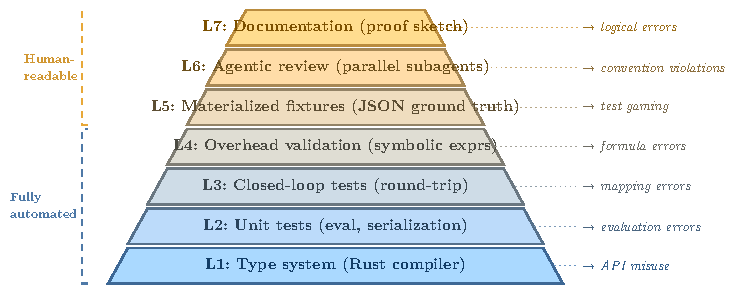
\includegraphics[width=\columnwidth]{figures/verification-pyramid.pdf}
  \caption{Seven-layer verification stack. Lower layers (blue) are fully automated and fast; upper layers (gold) involve human-readable arguments and fresh-context review.}
  \label{fig:verification}
\end{figure}

\paragraph{Layer 1: Type system.}
The \texttt{Problem} trait's associated type forces every problem to declare whether it is an optimization or decision problem.
The overhead macro validates variable names against source-type methods.
Errors are caught in seconds, before any test runs.

\paragraph{Layer 2: Unit tests.}
Each problem includes tests verifying \lstinline{evaluate()} on small, hand-crafted instances.
Serialization round-trip tests catch graph and weight encoding issues.

\paragraph{Layer 3: Closed-loop (round-trip) tests.}
The pattern described in \Cref{sec:roundtrip} exercises the full mathematical content of each reduction.
This catches index errors, sign errors, and mapping bugs---the largest share of errors that survive type checking.

\paragraph{Layer 4: Overhead validation.}
After constructing the target instance, the test harness evaluates the symbolic overhead expressions and compares the predicted sizes against the actual target sizes.
This is particularly effective for non-obvious size relationships (e.g., quadratic edge counts in intersection graphs that an agent might assume are linear).

\paragraph{Layer 5: Materialized fixtures.}
JSON ground-truth files in \texttt{tests/data/} are committed separately from implementations.
If an agent modifies a ground-truth file to make a test pass, the change appears as a visible diff in a file outside the agent's normal scope, transforming a subtle correctness violation into an obvious process violation.

\paragraph{Layer 6: Agentic review.}
Two parallel sub-agents---one checking structural completeness, one checking code quality---operate in fresh context windows.
Fresh context prevents the confirmation bias that arises when an agent reviews its own work within the same session.

\paragraph{Layer 7: Documentation and visual review.}
Every reduction has an entry in the accompanying paper with a proof sketch and a worked example.
The example is not manually drawn: it is generated by the same code that the round-trip test (Layer~3) executes.
The contributor specifies the source instance in the issue; the implementation produces JSON containing the source, target, overhead expressions, and extracted solutions; the paper renders this JSON as a visual diagram.
Contributors can inspect the paper to verify that the reduction matches their mathematical intent---a visual check that complements the automated verification layers below.
A completeness checker flags undocumented graph elements, ensuring every edge in the graph has a corresponding proof sketch.

\paragraph{The lazy agent problem.}
We observed agents modifying expected test outputs rather than fixing implementations---a rational strategy from the agent's perspective (shortest path to passing tests), but a correctness violation.
Layer~5's independent fixtures and Layer~6's fresh-context review are the primary defenses against this failure mode.

\section{Graph Topology Analysis}\label{app:topology}

The \texttt{topology-sanity-check} skill detects three categories of graph quality issues (\Cref{fig:topology}).

\begin{figure}[t]
  \centering
  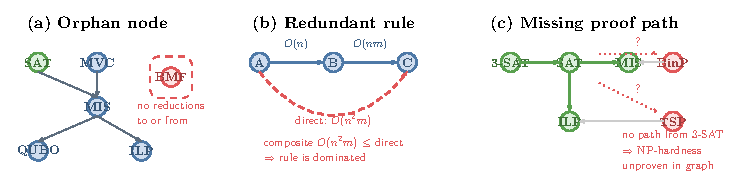
\includegraphics[width=\columnwidth]{figures/topology-issues.pdf}
  \caption{Three graph topology issues.
    \textbf{(a)}~An orphan node has no edges and cannot reach any solver.
    \textbf{(b)}~A direct reduction is redundant when a composite path through~$B$ has equal or lower overhead.
    \textbf{(c)}~Problems without a path from 3-SAT lack a machine-verifiable NP-hardness proof in the graph.}
  \label{fig:topology}
\end{figure}

\emph{Orphan nodes} contribute nothing to the graph's routing capability.
\emph{Redundant rules} waste implementation effort when a cheaper composite path exists.
\emph{Missing proof paths} indicate problems whose NP-hardness is not machine-verifiable within the graph.
The agent uses these categories to rank proposals by priority: rules that connect orphans or fill proof-chain gaps are suggested first.

\section{Ablation Study Design}\label{app:ablation}

To isolate the effect of skills on development outcomes, we design a controlled comparison on identical tasks.

\paragraph{Setup.}
Select 5--10 reductions spanning the complexity spectrum---from complement relationships (MVC $\to$ MIS, 96~lines) through gadget constructions (Satisfiability $\to$ MIS, 171~lines) to circuit encodings (Factoring $\to$ CircuitSAT, 272~lines).
Prepare identical issues for two configurations:
(1)~\emph{Skill-based}: the full pipeline including issue validation, implementation skills, multi-agent review, and CI fixing.
(2)~\emph{No-skill baseline}: the same agent, same codebase, and same project instructions, but no skill files---the agent must infer the workflow from context.

\paragraph{Metrics.}
(1)~First-attempt CI pass rate; (2)~review rounds before merge readiness; (3)~correctness (all round-trip tests pass); (4)~convention adherence (file naming, macro usage, documentation completeness).

\paragraph{Expected outcomes.}
Skills should excel on convention adherence (encoding project-specific patterns that are not inferrable from code alone) and first-attempt CI pass rate (the verification stack catches errors before the pull request is created).
The baseline agent likely produces functionally correct code that fails CI due to missing macros, incorrect overhead declarations, or misplaced test files.

This ablation has not yet been executed.
We present the design as a replicable protocol for evaluating skill-based methodologies.

\end{document}
